\subsection{Результаты экспериментов и анализ данных}

\subsection*{Условия проведения эксперимента}

В рамках экспериментальной проверки работы имитатора было сгенерировано
и последовательно поставлено в очередь диспетчера $N = 783$ синтетических
заявок. Все четыре вычислительных узла кластера
(\texttt{node1}--\texttt{node4}) на момент начала эксперимента находились
в состоянии полной готовности (\texttt{idle}), управляющий узел
\texttt{master} успешно координировал распределение ресурсов.

\subsection*{Результаты постановки заявок в очередь}

По завершении выполнения всех сгенерированных задач из базы данных
подсистемы учёта SLURM и логов имитатора были собраны итоговые
статистические характеристики. Сводные результаты сопоставления плановых
параметров и фактических метрик выполнения для первых пяти заявок
представлены в таблице~\ref{tab:results}.

\begin{table}[H]
\caption{Пример сравнения плановых и фактических характеристик выполнения заявок}
\label{tab:results}
\centering
\begin{tabular}{|c|c|c|c|c|}
\hline
SlurmJobID & $T_{\text{заявки}}$ (план), с & $T_{\text{факт}}$, с & Узлов & Состояние \\
\hline
2657 & 1495 & 23 & 3 & COMPLETED \\
2656 & 2210 & 34 & 1 & COMPLETED \\
2658 & 1421 & 29 & 3 & COMPLETED \\
2659 & 1127 & 23 & 2 & COMPLETED \\
2660 & 1029 & 21 & 3 & COMPLETED \\
\hline
\end{tabular}
\end{table}

\subsection*{Анализ отклонений «план -- факт»}

Сопоставление запрошенного пользователем времени выполнения
$T_{\text{заявки}}$ и фактического времени выполнения $T_{\text{факт}}$
выполнено по результатам эксперимента с $N = 783$ заявками.
Из общего числа заявок 47~(6{,}0\,\%) были поданы с лимитом времени,
заведомо меньшим фактического, что соответствует теоретической
вероятности таймаута $p_{\text{timeout}} = 0{,}05$. Для оставшихся
736~нормальных заявок по значениям $T_{\text{заявки}}$ и $T_{\text{факт}}$
вычислены выборочные логарифмы коэффициента
$\tau = T_{\text{заявки}} / T_{\text{факт}}$, на основе которых получены
эмпирические оценки параметров логнормального распределения~\cite{kappes2018userestimates, sherrill2023hpcruntime}:
$\hat{\mu} = 3{,}8973$ и $\hat{\sigma} = 0{,}8578$.

Полученные значения демонстрируют высокую степень близости к теоретическим
параметрам, использованным при генерации: $\mu = 3{,}8621$ и
$\sigma = 0{,}8489$. Относительное отклонение по параметру $\mu$ составляет
$0{,}9\,\%$, по параметру $\sigma$ --- $1{,}1\,\%$, что подтверждает
статистическую адекватность разработанной модели при объёме выборки
$N = 783$.

По данным файла учёта заданий SLURM, фактическое время выполнения задач
находится в диапазоне от~2 до~43~секунд при среднем значении 22{,}5~с и
стандартном отклонении 9{,}4~с, что соответствует заданным границам
модельного диапазона $[T_{\min},\, T_{\max}] = [1,\, 43]$~с.
Визуальное сопоставление эмпирических распределений коэффициента ошибки
$\tau$ для исторических и сгенерированных данных представлено на
рисунке~\ref{fig:error_distributions}.

% \begin{figure}[H]
%     \centering
%     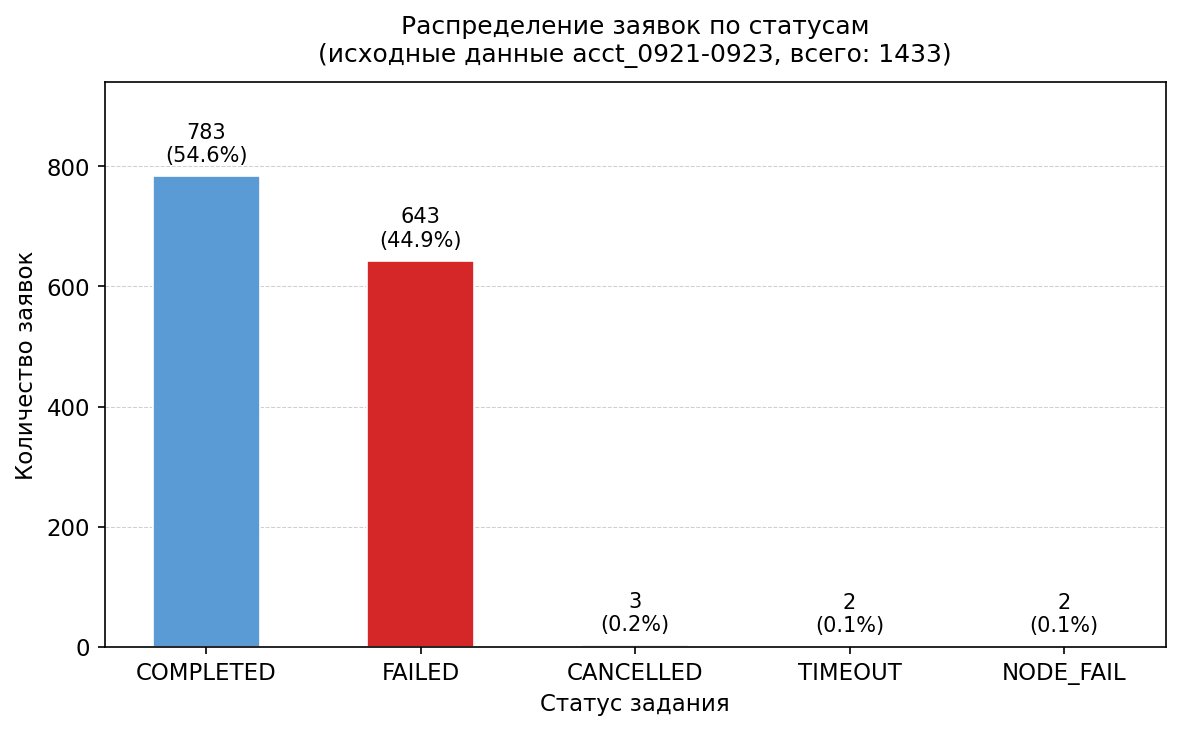
\includegraphics[width=1\textwidth]{figures/fig1a_raw_states.png}
%     \caption{Распределение заявок по статусам (исходные данные)}
%     \label{fig:fig1a}
% \end{figure}


% \begin{figure}[H]
%     \centering
%     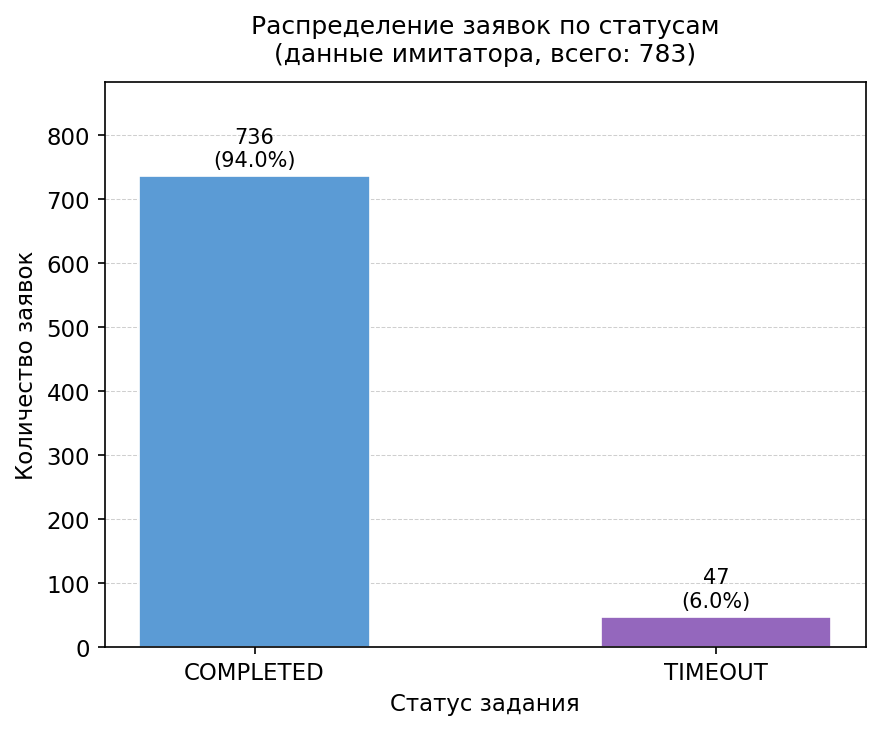
\includegraphics[width=0.9\textwidth]{figures/fig1b_sim_states.png}
%     \caption{Распределение заявок по статусам (данные имитатора)}
%     \label{fig:fig1b}
% \end{figure}

\begin{figure}[H]
    \centering
    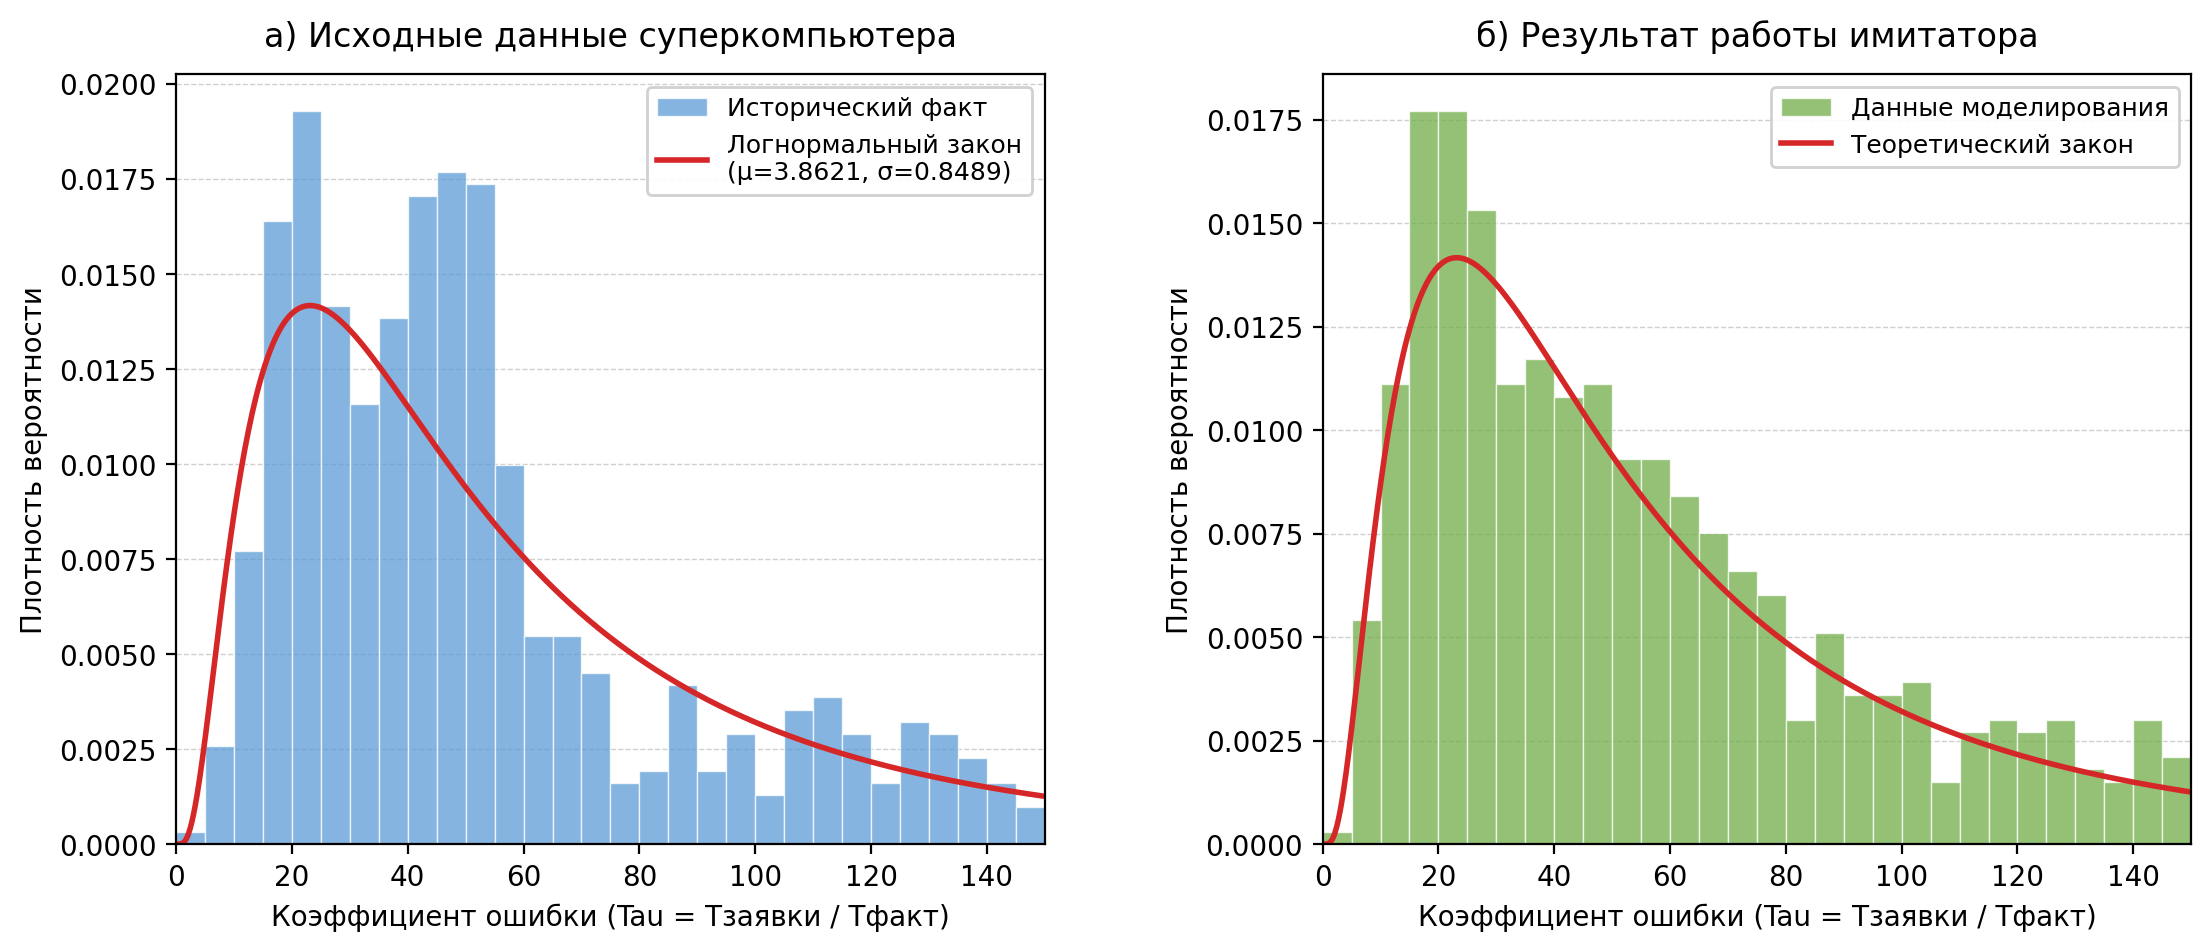
\includegraphics[width=1\textwidth]{figures/error_distributions.png}
    \caption{Плотность распределения коэффициента ошибки пользователя
    $\tau$: а)~на основе исторических данных выборки acct\_0921-0923;
    б)~сгенерированная программным имитатором}
    \label{fig:error_distributions}
\end{figure}

\subsection*{Выводы по результатам экспериментов}
Проведённый эксперимент показал, что разработанный имитатор
пользовательских заявок на языке \texttt{Python~3} обеспечивает корректную
автоматическую постановку заданий в очередь диспетчера SLURM. Все
783~сгенерированные заявки были успешно приняты планировщиком и выполнены
на вычислительных узлах кластера. Статистические характеристики
сгенерированной нагрузки --- эмпирические оценки параметров логнормального
распределения $\hat{\mu} = 3{,}8973$ и $\hat{\sigma} = 0{,}8578$ ---
воспроизводят теоретические параметры исходной выборки с отклонением менее
$1{,}2\,\%$. Это подтверждает применимость предложенного статистического
подхода к моделированию пользовательской нагрузки на вычислительный кластер
при отсутствии доступа к данным реальной эксплуатационной системы в
реальном масштабе времени.